% ============================================================================================
% Section 8 (revised): Experimental Evaluation. Numbers are read from results/final/*.json and
% results/revision_2/*.json; figures and generated tables come from paper/make_eval_r2.py.
% ============================================================================================
\section{Experimental Evaluation}
\label{sec:ev}

This section evaluates \pamcp{} along the four research questions of Section~1. Section~\ref{sec:ev-setup} fixes
the data, the compared methods, the varied parameters and the statistical protocol. The next five subsections
answer RQ1 (representation and model-conditioned gap, Section~\ref{sec:ev-rq1}), RQ2 (trust under missing, forged
and imperfect evidence, Section~\ref{sec:ev-rq2}), RQ3 (retrieval, toolkit quality and certification,
Section~\ref{sec:ev-rq3}), the security behaviour and the contribution of each mechanism
(Section~\ref{sec:ev-sec}), and cost, scalability, adaptation and stability (RQ3/RQ4,
Section~\ref{sec:ev-eff}). Section~\ref{sec:ev-threats} states the limits of the evidence. Every subsection
gives the protocol, a results table, figures, the observations and their interpretation, and compares
\pamcp{} with baselines wherever a baseline exists.

\subsection{Experimental Setup}
\label{sec:ev-setup}

\emph{Evidence classes.} The claims of the paper differ in what can establish them. We label every result with
one of six evidence classes: \emph{formal} (a proof in Sections~5--7), \emph{simulated} (generated under stated
assumptions, e.g.\ a verifier with a controlled error rate), \emph{labelled} (scored against machine-generated
reference labels), \emph{measured} (obtained from the running implementation against benchmark gold or solver
optima), \emph{observed} (from controlled execution traces of real MCP servers) and \emph{human-validated}.
Fig.~\ref{fig:ev-evidence} maps each claim to the classes that support it. Two claims have no supporting
evidence in this study: end-to-end task success of executed toolkits and human-validated contracts; no
conclusion below rests on them.

\begin{figure}[t]
\centering
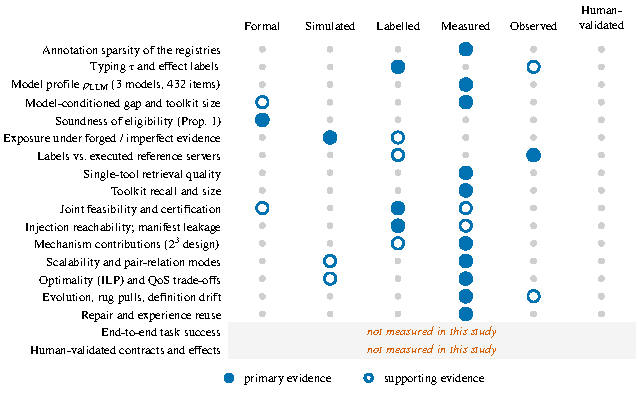
\includegraphics[width=\columnwidth]{fig_setup_evidence}
\caption{Evidence map: the class of evidence behind each claim evaluated in this section (filled: primary,
open: supporting). Shaded rows are not measured.}
\label{fig:ev-evidence}
\end{figure}

\emph{Registries and tasks.} Table~\ref{tab:ev-data} lists the data. The registry merges LiveMCPTool
\cite{mo2025livemcpbench} and the tool set of MCPToolBench++ \cite{fan2025mcptoolbench} by
\texttt{server::name} (76 servers, 569 tools; Fig.~\ref{fig:ev-registry}a). Only 44 tools carry MCP annotations,
all of them \texttt{readOnlyHint=true}, and one of these is not read-only (Fig.~\ref{fig:ev-registry}c);
119 of the 525 unannotated tools are not read-only. Multi-step tasks are the 95 public LiveMCPBench tasks (94 with
a resolvable gold tool). Single-tool retrieval uses MCPToolBench++ requests: a 60-request development split (ten
per category) for every tuning decision, and a disjoint test sample of 300 requests (50 per category, 66 target
tools). Security and ablation experiments use 155 tasks (the 95 LiveMCPBench tasks and the 60 development
prompts), each under its least-privilege policy and under a strict read-only policy; confirmatory tests use the
test tasks only.

\begin{table}[t]
\centering
\caption{Data, splits and their use.}
\label{tab:ev-data}
\scriptsize
\setlength{\tabcolsep}{3pt}
\begin{tabular}{@{}p{2.45cm}rp{4.55cm}@{}}
\toprule
Data & Size & Use \\
\midrule
Merged registry & 569 / 76 & tools / servers; 44 annotated; all experiments \\
LiveMCPBench tasks & 95 & multi-step test tasks (94 with gold tool) \\
MCPToolBench++ dev & 60 & tuning of every method (10 per category) \\
MCPToolBench++ test & 300 & single-tool retrieval (50 per category, 66 targets) \\
Security task set & 155 & 95 test tasks + 60 dev prompts, two policies \\
Calibration suite & 432 & 6 operations $\times$ 4 sizes $\times$ 2 languages $\times$ noise $\times$ context; 264 calibration / 168 test items, 3 models \\
Reference servers & 6 / 38 & servers / registry tools executed under tracing \\
Cloned registries & $10^3$--$10^5$ & near-copies of real contracts (scaling) \\
Heterogeneous registries & $10^3$--$10^5$ & generator varying servers, effects, sparsity, vocabulary, duplicates \\
Cover instances & 80 & 8 families $\times$ 10; exact optima by ILP \\
QoS instances & 120 & 4 roles $\times$ 4 providers; 4 weightings $\times$ 3 floors \\
\bottomrule
\end{tabular}
\end{table}

\begin{figure*}[t]
\centering
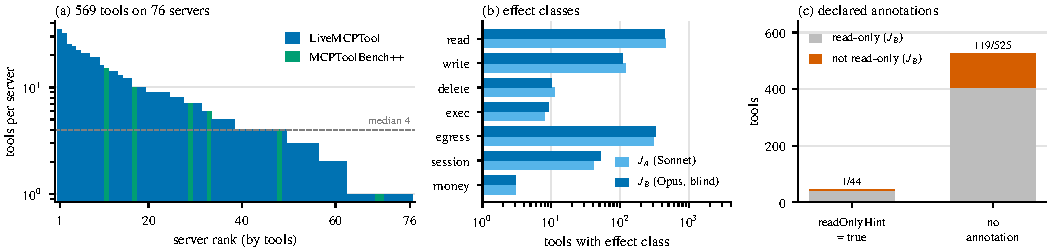
\includegraphics[width=\textwidth]{fig_setup_registry}
\caption{The evaluation registry. (a) Tools per server (log scale). (b) Effect classes under the two LLM
labellings. (c) Declared annotations against the read-only status under $J_B$ (numbers: not read-only / total).}
\label{fig:ev-registry}
\end{figure*}

\emph{Reference labels.} Neither benchmark labels effects or types. Labels $J_A$ (Claude Sonnet, from name,
description and schema under a fixed guide) give the typing $\tau$ and drive the simulated verifier bound to
$h(t)$; labels $J_B$ (Claude Opus, blind, separate guide) are used for scoring
(Fig.~\ref{fig:ev-registry}b). They agree on state modification for 558 of 569 tools ($\kappa=0.944$). Because
every tool that is unsafe under $J_B$ (120) is also unsafe under $J_A$ (131), a verifier simulated from $J_A$ can
never admit a tool that $J_B$ calls unsafe; we therefore also report the swapped direction
(Section~\ref{sec:ev-rq2}) and compare both labellings with executed servers. All LLM outputs (analyst goal
contracts, MCP-Zero requests, COLT training queries, ToolScope merge judgements, calibration answers) were
recorded once and are replayed.

\emph{Compared methods.} Table~\ref{tab:ev-methods} lists the methods and what each may use. \pamcp{}
combines three mechanisms that the ablations switch independently: the model-conditioned gap (G,
Algorithm~1), provenance-sound eligibility (P, Section~5) and set-level reasoning with certification (S:
backward closure, minimum-cost cover, certificate; Section~6). \pamcp{}-L is the relevance-first variant
selected on the development split (lexical candidate ranking; structural matching only as a recorded,
uncertain constraint). The baselines are adapted to the common registry and share one dense encoder (TF-IDF with
truncated SVD); they are adaptations, not the published systems. Every retrieval method was tuned on the
development split with a comparable grid (Table~\ref{tab:ev-params}).

\begin{table}[t]
\centering
\caption{Compared methods: information used and tuning on the development split.}
\label{tab:ev-methods}
\scriptsize
\setlength{\tabcolsep}{2.5pt}
\begin{tabular}{@{}lp{3.95cm}c@{}}
\toprule
Method & Information used & Grid \\
\midrule
\pamcp{} & analyst goal contracts, typing $\tau$, evidence, profile, Eq.~(6) & 14 \\
\pamcp{}-L & as \pamcp{}; lexical ranking first, types as constraint & (sel.) \\
RAG-MCP \cite{gan2025ragmcp} & raw request, dense top-$k$ & 1 \\
BM25 / RRF fusion & raw request, lexical / lexical+dense & 12 / 4 \\
MCP-Zero \cite{fei2025mcpzero} & model-written requests, server routing & 4 \\
COLT \cite{qu2024colt} & query--scene--tool graph of 450 training queries & 16 \\
ToolScope \cite{liu2026toolscope} & LLM-confirmed tool merging, analyst subqueries & 3 \\
CMTF \cite{suresh2026cmtf} & typed-state search, one tool per step & 4 \\
Per-subtask & analyst subgoals, one tool each & -- \\
Full catalogue & all 569 tools & -- \\
\bottomrule
\end{tabular}
\end{table}

\emph{Varied parameters.} Table~\ref{tab:ev-params} lists every parameter that an experiment varies, with its
range and default; parameters not listed keep the values of Section~6.

\begin{table}[t]
\centering
\caption{Parameters varied in the experiments (default in bold).}
\label{tab:ev-params}
\scriptsize
\setlength{\tabcolsep}{2.5pt}
\begin{tabular}{@{}lp{4.2cm}l@{}}
\toprule
Parameter & Values & Section \\
\midrule
Candidate budget $K$ & 1, 5, \textbf{10}, 20, 40 & \ref{sec:ev-rq3}, \ref{sec:ev-eff} \\
Relevance weight $w_{\mathrm{rel}}$ & 0, 1, 3, \textbf{10} & \ref{sec:ev-rq3} \\
Profile threshold $\tau$ & 0.6, 0.75, \textbf{0.9}; risk targets 0.05, 0.10 & \ref{sec:ev-rq1} \\
Input size $n$ & 10, 30, 40, 160, 300, 640, 3k, 30k & \ref{sec:ev-rq1} \\
Forging servers $\delta$ & 0, 0.05, 0.1, 0.2, 0.3 (5 seeds each) & \ref{sec:ev-rq2} \\
Verifier false accept $\varphi$ & 0, 0.01, 0.02, \textbf{0.05}, 0.1, 0.2 & \ref{sec:ev-rq2} \\
Probe coverage $\kappa$ & 0.25, 0.5, 0.75, \textbf{1} & \ref{sec:ev-rq2} \\
Trust threshold $\ell_{\min}$ & 0.2--0.95 (step 0.05), \textbf{0.65} & \ref{sec:ev-rq2} \\
Poisoned descriptions & 0, 10\%, 30\% of tools & \ref{sec:ev-sec} \\
Mechanisms G, P, S & on/off ($2^3$) + 5 components & \ref{sec:ev-sec} \\
Registry size & 569, $10^3$, $10^4$, $10^5$ tools & \ref{sec:ev-eff} \\
Pair relation & \textbf{eager}, partitioned, lazy & \ref{sec:ev-eff} \\
Cost weights $\beta,\gamma,\delta,\eta,\zeta$ & 0, 0.25, \textbf{0.5}, 1 & \ref{sec:ev-eff} \\
Utility floor $u_{\min}$ & 0, 0.4, \textbf{0.5}, 0.6, 0.8, 0.9 & \ref{sec:ev-eff} \\
Node budget (exact search) & \textbf{20,000} & \ref{sec:ev-eff} \\
\bottomrule
\end{tabular}
\end{table}

\emph{Statistical protocol.} Request-level metrics are resampled with target tools as clusters and task-level
metrics with tasks as clusters; paired comparisons use two-sided sign-flip permutation tests on cluster sums,
proportions use Wilson intervals, and all intervals are 95\%. Two confirmatory families were fixed before the
data they test were seen: seven comparisons F1--F7 (before the set-level experiments) and an amendment H1--H5
(committed, dated, before any test-set run of the revised analyses), each with Holm correction and, for recall, a
non-inferiority margin of 0.05. All other comparisons are exploratory and reported as such. Code, recorded LLM
outputs, per-item results, run manifests (commit, input and label hashes, package versions) and a notebook that
re-runs every experiment on a CPU runtime are
available.\footnote{\url{https://github.com/msellamiTN/taas-provenance-discovery}, branch
\texttt{research/pamcp-final-evaluation}.}
